
\section{Motivation}

The motivation for this thesis mainly includes two parts, in the first part, we illustrate the roots of container-based server consolidation problem. In the second parts, we explain the motivations for solving the sub-problems of the problem.

\subsection{Motivation For Container-based Server Consolidation Problem}

\begin{enumerate}
\item Container is a new virtualization technology which provides an operating level of virtualization.
Figure \ref{fig:root} illustrates the root of container technology from an energy efficient point of view. Most Clouds provide a set fixed types of VM for service providers to choose. Each type of VM represents a certain amount of resources (e.g. CPU, RAM, and Storage). This service model leads to a great waste of resources for two reasons. 
\begin{itemize}
	\item Firstly, service providers tend to over estimate the resources for ensuring the QoS at the peak hours, hence, they often reserve more resources \cite{Chaisiri:2012cv}. 
	\item Secondly, specific types of application may use a type of resources a lot more than another \cite{Tomas:2013iv}, for example, computation intensive tasks consume CPU much more than RAM; a fixed type of VM may provide much more RAM than it needs.
\end{itemize}
In order to solve this problem, overbooking strategy tends to place more VMs than the server's maximum capacity. However, this technique is highly relied on workload prediction on the application running in a VM. Otherwise, servers are easily overloaded. Container technique can improve the utilization by further partitioning VM into resource isolated chunks. Therefore, multiple applications can share the same VM. This technique avoids the prediction of workload as well as improving the utilization. 

Despite the potential improvement in energy efficiency, containers have advantages on other aspects. In terms of resource utilization, traditional IaaS (Infrastructure as a Service) Cloud data centers run many redundant operating systems and hypervisors. These redundancies can be eliminated by running multiple containers in a same operating system. From service model's perspective, softwares running in PaaS (Platform as a  Service) must be compatible with the platform: all technologies including programming languages, libraries must be supported by the platform. CaaS enhances PaaS by providing separated software runtime environment. These advantages make the container technology a popular trend. This is the reason that attracts us to
do research in this field.

\begin{figure}
	\centering
	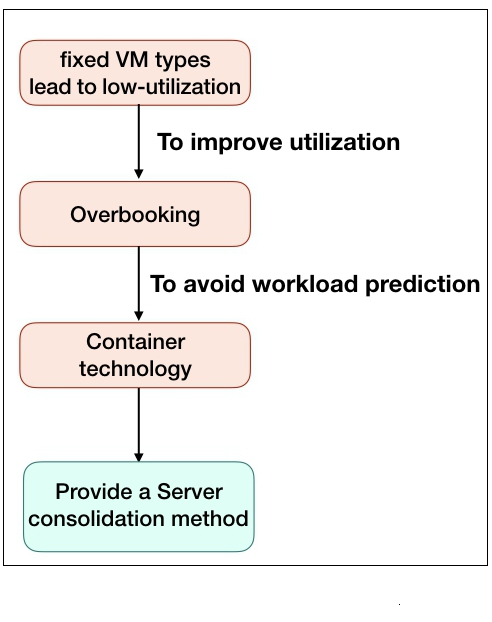
\includegraphics[width=0.3\textwidth]{pics/problem_flow.jpeg}
	\caption{The root of container technology}
	\label{fig:root}
\end{figure}

\item This container technology certainly brings many advantages to current Cloud industry\cite{Felter:2015ki}. However, it also brings difficulties for server consolidation. Server consolidation problems are typically modeled as vector bin-packing problem which are NP-hard. Container-based server consolidation adds another level of abstraction which makes it a two-level vector bin-packing problem. Current server consolidation methods are mostly VM-based which can not be directly applied on this problem, because two-level of bin-packing problems interact with each other. Piraghaj \cite{Piraghaj:2016bw} proposes a two-step procedure; it first maps tasks to VMs and then allocate containers to VMs. As Mann illustrated in \cite{Mann:2016hx},  these two steps should be conducted simultaneously, otherwise it leads to local optimal. Other research \cite{Dong:2014iz, Hindman:2011ux, Anselmi:2008ik} propose greedy-based heuristics on container allocation problem. They are fast in execution, but they can be easily stuck at local optimal. 
Therefore, it motivates us to provide \emph{global optimized} resource allocation solution for container-based data centers.

\end{enumerate}


\subsection{Motivation For Research Objectives}
The container-based consolidation problem, similar to VM-based consolidation, can be seen as 
a continuous optimization procedure with several stages. The goals for different stages are distinct, therefore, they can be seen as separate research questions. In this thesis, we aims at providing an end-to-end solution to the problem. Therefore, we divide the procedure into three stages: initialization, offline static optimization and online dynamic optimization stage. In addition to these three research questions, a scalability problem of static optimization is also considered as an objective.

\begin{enumerate}
\item In a CaaS cloud model, the initialization stage can be seen as a joint allocation of containers and virtual machines. This joint allocation is key step in ensuring energy efficiency.
At the initial stage, a set of containers is allocated to empty VMs and these VMs are allocated to physical servers. This seemingly two-step procedure is interconnected, therefore, should be conducted simultaneously. Because previous research \cite{Jennings:2015ht} focus on VM-based optimization, new problem models, including price and power model, constraints, and optimization objectives,  are the primary issue. In the second step, we will consider different representations and algorithms for solving this problem.

\item Server consolidation can be considered as static or dynamic problem \cite{Xiao:2015ik}.
Cloud data center has a highly dynamic nature with arrival and release of VMs. Therefore, 
after the initial allocation, the energy efficiency keeps dropping.  At a certain time point, e.g. a fixed time interval, a \emph{static server consolidation} is conducted to improve the global energy efficiency. Similar with VM-based consolidation, the problem is considered as a multi-objective problem with minimization of migration cost as well as keeping a good energy efficiency. Distinct from previous studies, the problem model has become a two-level of bin-packing problem which both container and VM migration cost should be considered.  
% and representations must be proposed to capture the characteristic of the joint allocation. 
% 	and the VMs are allocated to physical machines in the second step. Because of the complexity, previous research
% 	only considers the first step. They map the incoming tasks into predefined categories and based on the characteristic of the categories, the size of new virtual machines' resources are decided. After each tasks have chosen its VM type, they are allocated to virtual machines using a lightweight heursitic algorithm. 
% 	We intend to apply an EC-based approach to solve this problem by proposing a coevolutionary that simuetiously decide the virtual machine type as well as the allocation of VMs.
\item Dynamic consolidation is another method to maintain a high energy efficiency. Unlike static consolidation is conducted periodically in a global scale, dynamic consolidation is applied on single VM or container at any time point.  At large, data center system monitors all the states of servers for overloaded and underloaded servers. Once an overloaded server is detected, one of the VM or container running inside the server will be migrated to other machine so that the applications do not suffer from a performance degradation; for an underloaded server, all its applications will be moved to other servers so that it can be turned off. In conclusion, the main goal for dynamic consolidation is to optimize the global energy consumption as well as prevent overloading.
In a container-based environment, it involves three steps . 
	\begin{itemize}
		\item \emph{When to migrate?} refers to determine the time point that a physical server is overloaded. 
		\item \emph{Which container to migrate?} refers to determine which container need to be migrated so that it optimize the global energy consumption.
		\item \emph{Where to migrate?} refers to determine which VM and host that a container is migrated to.  
	\end{itemize}
	Specifically, we focus on the third question: dynamic placement problem. Previous research employ simple heuristics \cite{Shi:2011ke, Forsman:2015ca, Beloglazov:2012ji}, they are fast but could not perform well. Multi-objective genetic algorithm (GA) \cite{Xu:2010vh} has been applied. However, GA is too slow for dynamic problem. 

	To solve a dynamic placement with large number of variables, heuristics and dispatching rules are often used\cite{Sarin:2011fu}.  In this scenario, a dispatching rule is considered as a function that determines the priorities of servers that a container can be placed. However, dynamic placement is much complex than bin-packing problem \cite{Mann:2015ua}. Therefore, we intend to develop a hyper-heuristic method - Genetic Programming (GP) technique \cite{Banzhaf:1998wc} or artificial immune system \cite{Hofmeyr:2000ju}- to automatic evolve dispatching rules to solve this problem. GP has been applied in generating dispatching rules for bin-packing problem \cite{Burke:2006ei, SoteloFigueroa:2013be} and it produces promising solutions.

\item Cloud data center typically has hundreds of thousands servers and more. 
	Large scale of server consolidation has always been a challenge. 
 	Many approaches have been proposed in the literature to resolve the problem. There are mainly two ways, both rely on distributed methods, hierarchical-based \cite{Jung:2010dt, Moens:2011gk} and agent-based management systems \cite{Yazir:2010bk}.
	The major problem in agent-based systems is that agents rely on heavy communication to maintain a high-level utilization. Therefore, it causes heavy load in the networking. Hierarchical-based approaches are the predominate methods. In essence, these approaches are static methods where all the states of machines are collected and analyzed. One of way to improving the effectiveness is to reduce the number of variables so that the search space is narrowed. In this thesis, we are going to investigate the way to eliminate the redundant information.
\end{enumerate}



% Traditional Cloud computing offers three services models: Infrastructure as a Service (IaaS), Platform as a Service (PaaS) and Software as a Service (SaaS). Both IaaS and PaaS describe how does a service provider use the cloud resources. The main difference of these two models are  
% IaaS allows service providers to manage the low-level details including the operating system and libraries. While, PaaS provides a higher level of abstraction where users only focus on the application development without caring the underlying operating system and system-level of resources such as CPU cores and memories. However, one drawback of PaaS is that cloud users must make sure their applications are complete compatible with the platform. And in many of the cases, it is not the situation. In order to solve this problem, a container-based virtualization technology starts to reform the Cloud industry. Container as a Service (CaaS) 
% is a new concept but it has been used in industry for many years. Containers provide an operating system-level of isolation environment for applications. It does not need a hypervisor but complete rely on the operating system. 


% This exciting new technology has bring so many advantages for both Cloud users and Cloud providers. From the providers' perspective, In a large system, running VMs means there are probably many same operating systems occupying memories and storages. Lightweight containers share operating system and therefore, there are more rooms for softwares. It increases the capability of Cloud data centers. Furthermore, in terms of resource utilization, it provides much finer granularity operation than a VM-based Cloud model. Containers partition
% a VM into smaller chunks so that with appropriate management, better energy efficiency can be achieved. From the cloud users' perspective, each container provides separated libraries for specific application.  Therefore, it does not contrained by the underlying platform. Like PaaS, Cloud users do not need to concern the scalability of applications. 
% Therefore, CaaS can potentially become one of the main stream in the future Cloud computing industry. 

% Secondly, energy-efficent computing has been the major concern since the begining of computers. Specifially, Cloud computing has become a popular form. Large-scale data centers have been built around the world. A data center can consume huge amount of energies and it needs to improve its energy-efficiency from multiple perspectives. As we discussed in the Introduction, computing servers are one of the major contribution to the energy consumption. 
% And according to observation by \cite{}, the average utilization resource are still very low which causes huge energy wastage. As we mentioned above, the container technolgy provides a better way of managing resources, it has the potential to largly improve the utilization than current VM-based Cloud model because it avoids some of the major drawbacks of VM-based model. 

% Thirdly, because the container technology is relatively new, previous research are mostly focus on IaaS model and so that the server consolidation has based on the VM-level. However,   

% Frist is this new technology of container that can potentially change the landscape of
% Cloud computing. It has so many benefits but also it brings difficulty in managing resources.

% Second, from green computing point of view, we still need to manage resource so that, the 
% data centers consume less energy. And container technolgy actually bring a better chance to
% be more energy-efficient than previous VM based technology.
% Third, it is very difficult to manage this container-based resources because of the problem-nature is too complicated. And existed algorithms can not be directly applied on it.
% Fourth, the evolutioanry computation provides a good framework to handle such difficult problem.

% \textcolor{Blue}{Motivation is what is now lack from the literature.} \\

% The advantage of Platform as a Service (PaaS) has been discovered in the recent years. 
% The disadvantage of tranditional IaaS model has been discovered in the recent years \cite{Mann:2016hx}.
% In IaaS, on one hand, cloud customers need to manage the low-level details ranging from application capacity estimation,
% resource planning and selection and deployment. 
% On the other hand, Cloud providers manage resource provisioning and allocation. 
% Although these two tasks are seemingly different, 


% The container as a Service (CaaS) cloud model has gain increasing attention in the recent years.
% However, the energy efficiency in CaaS cloud environment has not been investigate. 
% Particularly, the virtual machine and container joint consolidation is the core problem.
% Therefore, in this thesis, we will focus on the end-to-end energy-aware server consolidation on container-based
% Cloud. In the meanwhile,  a major research direction of large scale server consolidation is also considered. 
% The end-to-end server consolidation refers to the server consolidation techniques used
% in the different stages throughout the routine Cloud resource management including  initial VM provisioning and placement, dynamic VM placement, and static VM placement:
